\section{The kinematic edge}\label{sec:21.3}

A silicon detector that counts single electrons has no electron-recoil rate below the phonon-assisted onset, \SI{0.3374}{MeV} for free pairs (\cref{sec:13.1}), and just above it the rate grows as the $13/2$ power of the distance in mass (\cref{eq:13.9-medge}). In the model of \cref{fig:21-edge} the limit on $\sigmae$ is $1.6\times10^7$ times weaker \SI{0.001}{MeV} above the onset than at \SI{0.35}{MeV}, and still 4.6 times weaker \SI{0.010}{MeV} above it. Every mass up to \SI{0.010}{MeV} above the onset is tested only by particles within \SI{12}{km.s^{-1}} of $v_{\mathrm{max}}$, a fraction $6.0\times10^{-5}$ of the standard halo. The steep power, the position of the edge and its height therefore carry the halo model as much as the target. We will derive the power for any channel and any truncation of the halo, and work out which combinations of gap, threshold and halo parameters a limit near its edge measures.

\subsection{The rate kernel near its onset}\label{sec:21.3-kernel}

For a response averaged over the directions of $\vect{q}$, the rate is the speed integral $\mathcal{R} = (\rho_\chi/\mchi\rho_T)\int\dd v\, F_\chi(v)\,\varGamma(v)$ of \cref{sec:21.1-eta}. The kernel $\varGamma(v)$ of \cref{eq:21.1-gammav} vanishes below the onset speed $v_{\mathrm{on}}(\mchi)$ (\cref{sec:21.1-functional}), and the edge is decided by how it starts there. A particle of mass $\mchi$ and speed $v$ reaches the pair $(q,\omega)$ when $\vmin(q,\omega) \le v$, that is when $\omega \le qv - q^2/2\mchi$ (\cref{eq:1.3-vmin}). Let $E_{\mathrm{th}}(q)$ be the onset of the direction-averaged response at fixed $q = |\vect{q}|$, as in \cref{sec:13.9-onset}. We generalize the definition of \cref{sec:13.3} from the phonon-assisted loss function to any channel: the response rises above the onset as $x^{p_{\mathrm{on}}}$, with $x = \omega - E_{\mathrm{th}}(q)$. At fixed $q$ the energy integral then runs from $x = 0$ to the largest energy above the onset that the stream reaches,
\begin{equation*}
  x_{\mathrm{max}}(q; v) = qv - \frac{q^2}{2\mchi} - E_{\mathrm{th}}(q) ,
\end{equation*}
which is the $x_{\mathrm{max}}$ of \cref{sec:13.9-onset} with $v_{\mathrm{max}}$ replaced by $v$. The integral contributes $x_{\mathrm{max}}^{p_{\mathrm{on}}+1}/(p_{\mathrm{on}}+1)$ times the smooth factors of the channel: $F_{\mathrm{DM}}^2$, the powers of $q$ and the strength of the response.

The onset speed $v_{\mathrm{on}}(\mchi)$ is the speed at which the largest $x_{\mathrm{max}}$ reaches zero. Setting $v = v_{\mathrm{max}}$ and solving for the mass instead defines the edge mass of the channel,
\begin{equation}
  m_{\mathrm{edge}} = \min_q \frac{q^2}{2\,[qv_{\mathrm{max}} - E_{\mathrm{th}}(q)]} ,
  \label{eq:21.3-medge}
\end{equation}
which is \cref{eq:13.1-mPAdef} and \cref{eq:13.1-mZP} written for any onset. It reduces to $m_{\mathrm{min}}$ of \cref{eq:1.3-mmin} when $E_{\mathrm{th}}$ does not depend on $q$. Let $q^*$ be the optimal momentum transfer. Since $\partial x_{\mathrm{max}}/\partial v = q$, a stream slightly faster than $v_{\mathrm{on}}$ reaches $x_{\mathrm{max}}(q^*) = q^*(v - v_{\mathrm{on}})$ at the optimum, and near it
\begin{equation*}
  x_{\mathrm{max}}(q; v) \simeq q^*(v - v_{\mathrm{on}}) - \frac{(q - q^*)^2}{2\mchi} ,
\end{equation*}
where, as in \cref{sec:13.9-onset}, the curvature of $E_{\mathrm{th}}(q)$ is dropped against $1/\mchi$. That holds at the phonon-assisted onset; at the zero-phonon edge, where the onset rises steeply in $q$, the curvature changes the prefactor $\varGamma_{\mathrm{on}}$ below but not the exponent, which needs only a positive total curvature. The range of $q$ with $x_{\mathrm{max}} > 0$ has a width proportional to $(v - v_{\mathrm{on}})^{1/2}$, and the integral of $x_{\mathrm{max}}^{p_{\mathrm{on}}+1}$ over it is $(2\mchi)^{1/2}[q^*(v - v_{\mathrm{on}})]^{p_{\mathrm{on}}+3/2}B(\tfrac12, p_{\mathrm{on}}+2)$, with $B$ the Euler beta function. The kernel therefore starts as
\begin{equation}
  \varGamma(v) \simeq \varGamma_{\mathrm{on}}\,(v - v_{\mathrm{on}})^{p_{\mathrm{on}} + 3/2} , \qquad v \to v_{\mathrm{on}}^+ ,
  \label{eq:21.3-kernel}
\end{equation}
with a coefficient $\varGamma_{\mathrm{on}}$ that collects the strength of the response at the onset, $F_{\mathrm{DM}}^2(q^*)$ and the powers of $q^*$ and $\mchi$. The power $p_{\mathrm{on}} + 3/2$ counts $p_{\mathrm{on}} + 1$ from the energy integral and $\tfrac12$ from the width in $q$.

The $\tfrac12$ becomes 1 when $x_{\mathrm{max}}(q)$ has a corner at its maximum. If $x_{\mathrm{max}} \simeq x_{\mathrm{max}}(q^*) - s_\pm|q - q^*|$ with slopes $s_\pm$ on the two sides, the width in $q$ is linear in $v - v_{\mathrm{on}}$ and the power is $p_{\mathrm{on}} + 2$. A corner arises when the onset itself has a kink at $q^*$, or when the range of $q$ ends there. The second is the case of the free nuclear recoil with a detector threshold. Its response is the line $\omega = q^2/2M$, a delta function at fixed $q$, so the energy integral is a constant, which is the case $p_{\mathrm{on}} = -1$. The threshold cuts the range of momentum transfers at $q_{\mathrm{th}} = (2ME_{\mathrm{th}})^{1/2}$, and near the edge the optimum sits at that cut. The kernel of the free nuclear recoil therefore starts linearly, with power $-1 + 2 = 1$.

\subsection{The escape tail of the halo}\label{sec:21.3-tail}

The other factor of the speed integral, $F_\chi(v)$, vanishes at $v_{\mathrm{max}}$, and how it vanishes depends on how the galactic distribution goes to zero at the escape speed. The standard halo of \cref{tab:1-shm} is cut by hand (\cref{eq:1.2-fgal}), so the distribution in the galactic frame stays finite up to $v_{\mathrm{esc}}$ and then drops to zero. Equilibrium distribution functions built for the density profiles of simulated halos go to zero smoothly instead. Lisanti and co-workers write such a family as~\cite[Eq.~(1)]{lisanti2011dark}
\begin{equation*}
  f_{\mathrm{gal}}(u) \propto \left[\exp\!\left(\frac{v_{\mathrm{esc}}^2 - u^2}{k_{\mathrm{tail}}\,v_0^2}\right) - 1\right]^{k_{\mathrm{tail}}}\Theta(v_{\mathrm{esc}} - u) ,
\end{equation*}
which near the escape speed behaves as $(v_{\mathrm{esc}} - u)^{k_{\mathrm{tail}}}$~\cite[Eq.~(11)]{lisanti2011dark}. The \emph{tail exponent} $k_{\mathrm{tail}}$ is zero for the sharp cut of the standard halo and one for the King model, $f_{\mathrm{gal}} \propto \ee^{-u^2/v_0^2} - \ee^{-v_{\mathrm{esc}}^2/v_0^2}$~\cite[Eq.~(12)]{lisanti2011dark}. Their fits to the velocity distributions of simulated galactic halos prefer $k_{\mathrm{tail}}$ between 1.5 and 3.5~\cite[Sect.~II, Eq.~(10), and Fig.~3]{lisanti2011dark}. Near the escape speed, then, $f_{\mathrm{gal}} \simeq f_{\mathrm{esc}}\,y^{k_{\mathrm{tail}}}$ with $y = v_{\mathrm{esc}} - u$ and a constant $f_{\mathrm{esc}}$; for the standard halo $f_{\mathrm{esc}} = \ee^{-v_{\mathrm{esc}}^2/v_0^2}/N_{\mathrm{esc}}$, the height of the normalized distribution at the cut.

The laboratory speeds near $v_{\mathrm{max}} = v_{\mathrm{esc}} + v_{\mathrm{E}}$ come from a small cap of velocity space. The fastest particle has its galactic velocity antiparallel to $\vect{v}_{\mathrm{E}}$, so take the unit vector $\hat{\vect{e}} = -\vect{v}_{\mathrm{E}}/v_{\mathrm{E}}$ and write a laboratory velocity as $\vect{v} = (v_{\mathrm{max}} - s)\hat{\vect{e}} + \vect{v}_\perp$, with $s$ and $|\vect{v}_\perp|$ small. To second order in them the laboratory speed and the galactic speed are
\begin{equation*}
  v \simeq v_{\mathrm{max}} - s + \frac{v_\perp^2}{2v_{\mathrm{max}}} , \qquad
  u = |\vect{v} + \vect{v}_{\mathrm{E}}| \simeq v_{\mathrm{esc}} - s + \frac{v_\perp^2}{2v_{\mathrm{esc}}} .
\end{equation*}
A particle with $v \ge v_{\mathrm{max}} - \delta$ that is bound to the halo therefore has $0 \le y \le \delta - a_\perp v_\perp^2$, with $a_\perp = 1/2v_{\mathrm{esc}} - 1/2v_{\mathrm{max}} = v_{\mathrm{E}}/(2v_{\mathrm{esc}}v_{\mathrm{max}})$: a lens of depth $\delta$ and radius $(\delta/a_\perp)^{1/2}$. At fixed $\vect{v}_\perp$ the volume element is $\dd s = \dd y$, and the fraction of particles in the lens is
\begin{equation*}
  \int\!\dd^2v_\perp\int_0^{\delta - a_\perp v_\perp^2}\!\dd y\, f_{\mathrm{esc}}\,y^{k_{\mathrm{tail}}}
  = \frac{\pi f_{\mathrm{esc}}\,\delta^{k_{\mathrm{tail}}+2}}{a_\perp(k_{\mathrm{tail}}+1)(k_{\mathrm{tail}}+2)} .
\end{equation*}
Its derivative with respect to $\delta$ is the speed distribution at $v = v_{\mathrm{max}} - \delta$:
\begin{equation}
  F_\chi(v) \simeq F_{\mathrm{esc}}\,(v_{\mathrm{max}} - v)^{k_{\mathrm{tail}}+1} , \qquad
  F_{\mathrm{esc}} = \frac{2\pi f_{\mathrm{esc}}\,v_{\mathrm{esc}}v_{\mathrm{max}}}{(k_{\mathrm{tail}}+1)\,v_{\mathrm{E}}} ,
  \label{eq:21.3-tail}
\end{equation}
valid for $v_{\mathrm{max}} - v \ll v_{\mathrm{E}}, v_{\mathrm{esc}}$. Dividing by $v \simeq v_{\mathrm{max}}$ and integrating once more, $\eta(\vmin) \propto (v_{\mathrm{max}} - \vmin)^{k_{\mathrm{tail}}+2}$. For $k_{\mathrm{tail}} = 0$ this is the quadratic edge of \cref{eq:1.3-edge}, with its coefficient $A_\eta = \pi v_{\mathrm{esc}}\ee^{-v_{\mathrm{esc}}^2/v_0^2}/(v_{\mathrm{E}}N_{\mathrm{esc}}) = F_{\mathrm{esc}}/2v_{\mathrm{max}}$, so the lens reproduces the expansion of the closed form. For the smooth members the power law needs one more condition: the bracket of $f_{\mathrm{gal}}$ is linear in $y$ only for $y \ll k_{\mathrm{tail}}v_0^2/2v_{\mathrm{esc}}$, which is \SI{52}{km.s^{-1}} for the King model.

A smooth tail empties the lens. With the same $v_0$ and $v_{\mathrm{esc}}$, the $6.0\times10^{-5}$ of the standard halo within \SI{12}{km.s^{-1}} of $v_{\mathrm{max}}$, which decide every silicon mass up to \SI{0.010}{MeV} above the onset, become $4.7\times10^{-6}$ in the King model and $3.7\times10^{-8}$ for $k_{\mathrm{tail}} = 2.5$.

\subsection{The edge power law}\label{sec:21.3-power}

Both factors of the speed integral now start as powers, one at $v_{\mathrm{on}}$ and one at $v_{\mathrm{max}}$, and the integral is a beta function. Write $\delta_{\mathrm{on}} = v_{\mathrm{max}} - v_{\mathrm{on}}(\mchi)$ for the window of speeds that contribute. Inserting \cref{eq:21.3-kernel,eq:21.3-tail},
\begin{equation*}
  \begin{aligned}
  \mathcal{R} &\simeq \frac{\rho_\chi}{\mchi\rho_T}\,F_{\mathrm{esc}}\,\varGamma_{\mathrm{on}}\int_{v_{\mathrm{on}}}^{v_{\mathrm{max}}}\dd v\,(v_{\mathrm{max}} - v)^{k_{\mathrm{tail}}+1}(v - v_{\mathrm{on}})^{p_{\mathrm{on}}+3/2} \\
  &= \frac{\rho_\chi}{\mchi\rho_T}\,F_{\mathrm{esc}}\,\varGamma_{\mathrm{on}}\,B\bigl(k_{\mathrm{tail}}+2,\, p_{\mathrm{on}}+\tfrac52\bigr)\,\delta_{\mathrm{on}}^{\,p_{\mathrm{on}}+k_{\mathrm{tail}}+7/2} .
  \end{aligned}
\end{equation*}
The window is linear in the distance from the edge mass. The edge mass of \cref{eq:21.3-medge}, as a function of $v_{\mathrm{max}}$, changes by $\dd m_{\mathrm{edge}}/\dd v_{\mathrm{max}} = -q^{*3}/[2(q^*v_{\mathrm{max}} - E_{\mathrm{th}}(q^*))^2] = -2m_{\mathrm{edge}}^2/q^*$, since only the explicit dependence counts at the minimum. A mass $\mchi$ just above $m_{\mathrm{edge}}$ is therefore at its own edge for the speed $v_{\mathrm{on}} = v_{\mathrm{max}} - \delta_{\mathrm{on}}$ with
\begin{equation*}
  \delta_{\mathrm{on}} \simeq \frac{q^*}{2m_{\mathrm{edge}}^2}\,(\mchi - m_{\mathrm{edge}}) .
\end{equation*}
For a $q$-independent onset, $q^* = m_{\mathrm{min}}v_{\mathrm{max}}$ and this is the window $(v_{\mathrm{max}}/2)(\mchi - m_{\mathrm{min}})/m_{\mathrm{min}}$ of \cref{sec:1.3-edge}; at the phonon-assisted onset of silicon, \cref{eq:13.1-mPA} gives $q^* = m_{\mathrm{min}}^{\mathrm{PA}}(v_{\mathrm{max}} \pm u_\nu)$, with $u_\nu$ the group velocity of the phonon at $\vect{Q}^*$, equal to $m_{\mathrm{min}}^{\mathrm{PA}}v_{\mathrm{max}}$ up to $u_\nu/v_{\mathrm{max}} \sim 3\times10^{-3}$.

\begin{keyresult}[Edge power law]
Let the direction-averaged response of a channel rise as $x^{p_{\mathrm{on}}}$ above its onset, and let the galactic distribution of the halo vanish as $(v_{\mathrm{esc}} - u)^{k_{\mathrm{tail}}}$ at the escape speed. If the largest energy above the onset, $x_{\mathrm{max}}$, has a smooth maximum in $q$, the rate near the edge mass $m_{\mathrm{edge}}$ of \cref{eq:21.3-medge} is
\begin{equation}
  \mathcal{R}(\mchi) \propto (\mchi - m_{\mathrm{edge}})^{\,p_{\mathrm{on}} + k_{\mathrm{tail}} + 7/2} .
  \label{eq:21.3-power}
\end{equation}
If $x_{\mathrm{max}}$ has a corner, the power is $p_{\mathrm{on}} + k_{\mathrm{tail}} + 4$. The response contributes $p_{\mathrm{on}} + 1$, the width in $q$ one half (one at a corner), the halo $k_{\mathrm{tail}} + 1$, and the overlap of the two onsets one more. The power holds for either mediator, as long as $F_{\mathrm{DM}}$ is smooth at $q^* \neq 0$.
\end{keyresult}

For the standard halo, $k_{\mathrm{tail}} = 0$, \cref{eq:21.3-power} is \cref{eq:13.9-medge}. For the King model the silicon edge steepens from $13/2$ to $15/2$, and over the range preferred by simulated halos to between 8 and 10. The free nuclear recoil with a sharp threshold has a linear kernel and the power $3 + k_{\mathrm{tail}}$.

The power also sets how close to the edge an exposure reaches, the distance that \cref{sec:21.1-floor} left open. A background-free exposure excludes a mass at which it predicts more than 2.3 events (\cref{eq:1.5-N90}). Near the edge the predicted number is proportional to $M_{\mathrm{det}}t_{\mathrm{exp}}\sigmae(\mchi - m_{\mathrm{edge}})^{n}$, with the exposure $M_{\mathrm{det}}t_{\mathrm{exp}}$ and $n$ the power of \cref{eq:21.3-power}. At fixed $\sigmae$ the lowest excluded mass therefore lies at a distance from the edge proportional to $(M_{\mathrm{det}}t_{\mathrm{exp}}\sigmae)^{-1/n}$. At the free-pair edge of silicon, $n = 13/2$, ten times the exposure brings the excluded mass a factor $10^{-2/13} = 0.70$ closer to the edge; with the King tail the factor is 0.74.

\Cref{tab:21-edge} collects the powers of the silicon electron-recoil edges and the free nuclear recoil. The phonon-assisted entries use the onset exponents of \cref{sec:13.3,sec:13.8}. For the zero-phonon edge of \cref{sec:13.9-edges} the exponents follow from the counting rule of \cref{sec:13.3}: an isolated quadratic minimum in $D$ free variables gives $x^{D/2 - 1}$, and a vertex that vanishes linearly at the minimum adds one power. At fixed $|\vect{q}|$ a free zero-phonon pair has three free variables, the components of the hole's crystal momentum. The average over the two angles of $\hat{\vect{q}}$ adds two more, since each of the 24 equivalent optima of the first edge is an isolated minimum with curvatures $\beta_\theta$ and $\beta_z$ (\cref{sec:13.9-edges}). With $D = 5$ the pair would start as $x^{3/2}$. The first zero-phonon line, however, is second class: its vertex vanishes in the mirror plane and grows linearly with the distance from it (\cref{sec:13.9-glide}), so $p_{\mathrm{on}} = 5/2$. The Coulomb attraction lowers the onset exponent of a continuum at fixed $\vect{q}$ by one half, from $x^{1/2}$ to a step, as \cref{eq:13.8-edge} does for the phonon-assisted continuum, and the excitonic zero-phonon continuum has $p_{\mathrm{on}} = 2$. The $1s$ line is a delta function at fixed $\vect{q}$; the two angles turn it into a step and the vertex zero into $x^1$. Since the phonon-assisted rate is already open at \SI{0.405}{MeV}, these powers describe how the zero-phonon rate adds to the total, a kink in the rate rather than the edge of the limit.

\begin{table}[tbp]
  \caption{Powers of the rate in the dark-matter mass, $\mathcal{R} \propto (\mchi - m_{\mathrm{edge}})^{n}$, at the edges of silicon, for the sharp-cut standard halo ($k_{\mathrm{tail}} = 0$); a halo with tail exponent $k_{\mathrm{tail}}$ adds $k_{\mathrm{tail}}$ to every entry (\cref{eq:21.3-power}). Masses in MeV, with the halo of \cref{tab:1-shm}; $p_{\mathrm{on}}$ is the onset exponent of the direction-averaged response at fixed $|\vect{q}|$; the fourth column says whether $x_{\mathrm{max}}(q)$ has a smooth maximum or a corner at $q^*$ (\cref{eq:21.3-power}). The zero-phonon edges lie above the phonon-assisted onset, where they add a kink to the total rate. The nuclear-recoil row is for a \SI{10}{eV} threshold.}
  \label{tab:21-edge}
  \centering\small
  \begin{tabular}{@{}llccc@{}}
    \toprule
    Edge & $m_{\mathrm{edge}}$ & $p_{\mathrm{on}}$ & $x_{\mathrm{max}}$ at $q^*$ & $n$ \\
    \midrule
    Phonon-assisted, free pair (transverse acoustic) & 0.3374 & 3 & smooth & $13/2$ \\
    Phonon-assisted, excitonic continuum & 0.3374 & $5/2$ & smooth & 6 \\
    Phonon-assisted, exciton replica & 0.3332 & $3/2$ & smooth & 5 \\
    Zero-phonon, first edge, free pair & 0.405--0.408 & $5/2$ & smooth & 6 \\
    Zero-phonon, first edge, excitonic continuum & 0.405--0.408 & 2 & smooth & $11/2$ \\
    Zero-phonon, first edge, $1s$ line & 0.402--0.405 & 1 & smooth & $9/2$ \\
    Free nuclear recoil, sharp threshold & 137 & $-1$ & corner & 3 \\
    \bottomrule
  \end{tabular}
\end{table}

\Cref{fig:21-edge}(b) checks \cref{eq:21.3-power} in the model of \cref{sec:13.9-onset}: the computed transverse acoustic onset on the valley axis, a loss function $Cx^3$ and the family of halos above. The local power of the rate is $p_{\mathrm{on}} + k_{\mathrm{tail}} + 7/2$ to 0.002 up to \SI{3e-4}{MeV} above the onset for $k_{\mathrm{tail}} = 0$, 1 and 2.5. For the standard halo it drifts to 6.54 at \SI{0.005}{MeV} and 6.61 at \SI{0.02}{MeV}, as the curvature of the speed distribution enters; a light mediator leaves the power at 6.500 near the onset. The model loss function is the idealization. The computed one follows $x^3$ only for $x < \SI{1.3}{meV}$ (\cref{fig:13-paloss}), and since the largest energy above the onset grows as $x_{\mathrm{max}}^* = \tfrac12 v_{\mathrm{max}}^2(\mchi - m_{\mathrm{edge}})$, \SI{3.5}{meV} per \SI{0.001}{MeV}, the power is exact only within \SI{4e-4}{MeV} of the onset. At the zero-phonon edge, $x_{\mathrm{max}}^* = (q^{*2}/2m_{\mathrm{edge}}^2)(\mchi - m_{\mathrm{edge}})$ is \SI{5.3}{meV} per \SI{0.001}{MeV}; the $1s$ power holds while $x_{\mathrm{max}}^*$ stays below the exciton binding of \SI{14.7}{meV}, within \SI{0.0028}{MeV} of the line, and the continuum powers until neighboring optima merge \SI{49}{meV} above the edge (\cref{sec:13.9-rates}), \SI{0.009}{MeV} above it. The halo side is never the limitation at these masses: \SI{0.01}{MeV} above the onset the window is $\delta_{\mathrm{on}} = \SI{11.8}{km.s^{-1}}$, far inside the \SI{173}{km.s^{-1}} scale of the correction in \cref{eq:1.3-edge} and the \SI{52}{km.s^{-1}} range of the King tail.

\begin{figure}[tbp]
  \centering
  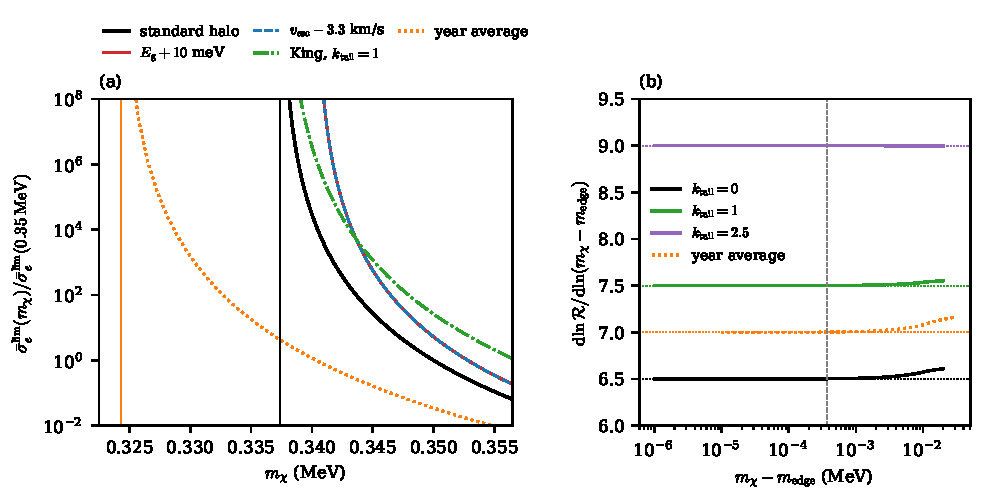
\includegraphics[width=\linewidth]{figures/ch21/fig21_3.pdf}
  \caption{The low-mass edge of a silicon electron-recoil limit. Model: direction-averaged loss function $Cx^3$ above the transverse acoustic onset on the valley axis ($m_{\mathrm{edge}} = \SI{0.33738}{MeV}$, PBE force constants of \cref{sec:5.2}, $\Eg = \SI{1.17}{eV}$), heavy mediator, background-free counting at fixed exposure, so that the limit is proportional to $1/\mathcal{R}$. (a)~Limit on $\sigmae$ relative to its value at \SI{0.35}{MeV}. Black: standard halo ($v_0 = 238$, $v_{\mathrm{esc}} = 544$, $v_{\mathrm{E}} = \SI{250.5}{km.s^{-1}}$). Red: gap raised by \SI{10}{meV}. Blue dashed, on top of the red curve: escape speed lowered by \SI{3.3}{km.s^{-1}} instead. Green dash-dotted: King model ($k_{\mathrm{tail}} = 1$) with the same $v_0$ and $v_{\mathrm{esc}}$. Orange dotted: an exposure spread uniformly over a year, with $v_{\mathrm{E}}$ between 237.4 and \SI{266.4}{km.s^{-1}}. Vertical lines: the edge at the reference speed and the June edge, \SI{0.3243}{MeV}. (b)~Local power of the rate, $\dd\ln\mathcal{R}/\dd\ln(\mchi - m_{\mathrm{edge}})$, for halos with tail exponents $k_{\mathrm{tail}} = 0$, 1 and 2.5 of the family of Lisanti and co-workers~\cite[Eq.~(1)]{lisanti2011dark} with the same $v_0$, $v_{\mathrm{esc}}$, $v_{\mathrm{E}}$, and for the year average ($m_{\mathrm{edge}}$ its June value). Dotted: the powers $p_{\mathrm{on}} + k_{\mathrm{tail}} + 7/2$ of \cref{eq:21.3-power} and $p_{\mathrm{on}} + 4$ for the year average. Dashed: the mass at which $x_{\mathrm{max}}^*$ reaches \SI{1.3}{meV}, the end of the $x^3$ range of the computed loss function.}
  \label{fig:21-edge}
\end{figure}

\subsection{Degeneracies at the edge}\label{sec:21.3-degeneracy}

Near its edge a limit is set by three numbers: the edge mass, the power and the height of the rate. Each is a combination of target and halo parameters, and parameters that enter the same combination cannot be told apart by the limit.

The edge mass depends on the onset $E_{\mathrm{th}}(q)$ and on $v_{\mathrm{max}} = v_{\mathrm{esc}} + v_{\mathrm{E}}$, and on nothing else. For a $q$-independent onset it depends on them only through $E_{\mathrm{th}}/v_{\mathrm{max}}^2$, the rule $\delta\ln m_{\mathrm{min}} = \delta\ln E_{\mathrm{th}} - 2\,\delta\ln v_{\mathrm{max}}$ of \cref{sec:1.3-edge}. The phonon-assisted onset of silicon depends on $q$, but \cref{eq:13.1-mPA} gives $m_{\mathrm{min}}^{\mathrm{PA}} = 2E_{\mathrm{on}}/(v_{\mathrm{max}}^2 - u_\nu^2)$ with the onset energy $E_{\mathrm{on}} = \Eg + \omega_\nu(\vect{Q}^*)$, and $u_\nu^2/v_{\mathrm{max}}^2 \sim 10^{-5}$. To that accuracy the edge measures the single ratio $E_{\mathrm{on}}/v_{\mathrm{max}}^2$. A one percent error in the onset energy $E_{\mathrm{on}}$, whether it comes from the gap, from the phonon energy that the onset adds or from the energy of a threshold of $n$ pairs, moves the edge exactly as a \SI{0.5}{\percent} change of $v_{\mathrm{max}}$, \SI{4.0}{km.s^{-1}}, does. Turned around, the escape-speed uncertainty of $\pm\SI{25}{km.s^{-1}}$ (\cref{sec:1.2}) moves the edge by $-6.0$ and $+6.6$ percent, as an error of $-71$ or $+78$~meV in the onset energy would, and the annual cycle of $v_{\mathrm{E}}$ by $-3.9$ and $+3.4$ percent.

The height of the rate is a product, $F_{\mathrm{esc}}\varGamma_{\mathrm{on}}$ in the speed integral above. The reference cross-section and the strength of the response at the onset sit in $\varGamma_{\mathrm{on}}$. The height $f_{\mathrm{esc}}$ of the galactic distribution at the cut and the geometric factor $v_{\mathrm{esc}}v_{\mathrm{max}}/v_{\mathrm{E}}$ of the lens sit in $F_{\mathrm{esc}}$. A null result near the edge bounds only the product. The dispersion $v_0$ enters the edge only here, through $f_{\mathrm{esc}}$: for the standard halo $\partial\ln A_\eta/\partial v_0 = 2v_{\mathrm{esc}}^2/v_0^3 - \partial\ln N_{\mathrm{esc}}/\partial v_0 = +\SI{3.2}{\percent}$ per km\,s$^{-1}$, so the uncertainty of $\pm\SI{6}{km.s^{-1}}$ (\cref{sec:1.2}) scales the rate near the edge by 1.21 and 0.83 at fixed edge mass. The escape speed enters both the edge mass and the height, but in the height its effect nearly cancels. At a fixed edge mass, lowering $v_{\mathrm{esc}}$ raises $A_\eta$ by \SI{1.76}{\percent} per km\,s$^{-1}$, since the cut moves into denser parts of the Maxwellian. It also lowers the powers of $v_{\mathrm{max}}$ in the rate. With the $q^3$ of \cref{eq:10.2-rate}, the energy integral of \cref{sec:13.9-onset} and $q^* = \mchi v_{\mathrm{max}}$, the rate at fixed $\mchi - m_{\mathrm{edge}}$ and fixed edge mass, with the gap moved together with $v_{\mathrm{esc}}$, scales as $A_\eta v_{\mathrm{max}}^{2p_{\mathrm{on}}+8}$ for a heavy mediator. For $p_{\mathrm{on}} = 3$ the factor $v_{\mathrm{max}}^{14}$ changes by \SI{1.76}{\percent} per km\,s$^{-1}$ as well, and the two changes cancel. A light mediator removes four powers of $v_{\mathrm{max}}$ through $F_{\mathrm{DM}}^2 \propto q^{*-4}$ and leaves \SI{0.5}{\percent} per km\,s$^{-1}$.

The power is a sum, $p_{\mathrm{on}} + k_{\mathrm{tail}}$, and the sum is all that a counting experiment can measure. The two exponents do enter the spectrum separately. At fixed $\omega$ the integral over $q$ of $\eta \propto (v_{\mathrm{max}} - \vmin)^{k_{\mathrm{tail}}+2}$, with $v_{\mathrm{max}} - \vmin = (x_{\mathrm{max}}(q) - x)/q$, runs over a range of width $\propto (x_{\mathrm{max}}^* - x)^{1/2}$ and gives
\begin{equation*}
  \frac{\dd\mathcal{R}}{\dd\omega} \propto (\omega - E_{\mathrm{on}})^{p_{\mathrm{on}}}\,(\omega_{\mathrm{top}} - \omega)^{k_{\mathrm{tail}} + 5/2} , \qquad \omega_{\mathrm{top}} = E_{\mathrm{on}} + x_{\mathrm{max}}^* ,
\end{equation*}
for an onset that is flat near $q^*$. The response shapes the bottom of the spectrum and the halo its top. The whole spectrum, however, is \SI{3.5}{meV} wide per \SI{0.001}{MeV} above the edge, while a silicon detector that counts pairs puts every deposit between $\Eg$ and $2\Eg$ into one bin (\cref{sec:1.5}). The bin integrates the spectrum, and with it the two exponents into their sum.

Two handles distinguish the target from the halo. The first is a second edge with a different mixture. At the zero-phonon edge the onset rises steeply with the distance of $\vect{q}$ from the valley, and the envelope theorem, by which only the explicit dependence of a minimized function on a parameter counts at its minimum (\cref{sec:21.3-power}), applied to \cref{eq:13.1-mZP} leads to $\partial\ln m_{\mathrm{min}}^{\mathrm{ZP}}/\partial\ln\Eg = \Eg/(q^*v_{\mathrm{max}} - E^*)$ and $\partial\ln m_{\mathrm{min}}^{\mathrm{ZP}}/\partial\ln v_{\mathrm{max}} = -q^*v_{\mathrm{max}}/(q^*v_{\mathrm{max}} - E^*)$, with $E^*$ the pair energy at the optimum and a rigid shift of the conduction bands. At the joint minimum of \cref{sec:13.9-edges}, $|\vect{q}^*| = \SI{1.33}{keV}$ and $E^* = \SI{1.355}{eV}$, these are 0.54 and $-1.62$, against 1 and $-2$ at the phonon-assisted onset. Two edges of one crystal measure the gap and $v_{\mathrm{max}}$ separately, in principle, although the zero-phonon edge appears only as a kink of the rate.

The second handle is time. Over the year $v_{\mathrm{max}}$ moves between 781 and \SI{810}{km.s^{-1}} (\cref{eq:1.2-vmax}) while the gap stays put, and near the edge the rate responds with the full power of \cref{eq:21.3-power}. An exposure spread over the year has the time-averaged rate. Near the largest Earth speed, on 2 June, the edge mass varies quadratically in time, $m_{\mathrm{edge}}(t) \simeq m_{\mathrm{edge}}^{\mathrm{June}} + \tfrac12\ddot m\,(t - t_{\mathrm{June}})^2$, and the time integral of $(\mchi - m_{\mathrm{edge}}(t))^{n}$ over the interval in which it is positive, of width $\propto (\mchi - m_{\mathrm{edge}}^{\mathrm{June}})^{1/2}$, adds one half to the power. The year-averaged edge sits at the June value, $m_{\mathrm{edge}}^{\mathrm{June}} = \SI{0.3243}{MeV}$ for the free-pair onset, \SI{3.9}{\percent} below the edge at the reference speed, with the power $p_{\mathrm{on}} + k_{\mathrm{tail}} + 4$ (\cref{fig:21-edge}(b)). At \SI{0.010}{MeV} above the reference edge the averaged rate is 62 times the rate at the reference speed, and at \SI{0.020}{MeV} still 8.5 times. Near the edge a limit computed at a fixed Earth speed is therefore a statement about that day (\cref{sec:21.1-floor}).

\begin{workedexample}{How a \SI{10}{meV} gap shift moves the silicon edge}\label{we:21-gapshift}
Ten meV is smaller than either energy that separates the silicon onsets, the exciton binding of \SI{14.7}{meV} and the transverse acoustic phonon at $\vect{Q}^*$, about \SI{15}{meV} (\cref{sec:13.1}). That phonon is softer than the \SI{18.27}{meV} replica of optical absorption, because the dark matter supplies part of the momentum and $\vect{Q}^*$ is shorter than the valley wavevector. Raise the gap by $\delta E = \SI{10}{meV}$, with the halo of \cref{tab:1-shm}.

\emph{Edge.} By \cref{eq:13.1-mPA}, $\delta m_{\mathrm{edge}} = 2\,\delta E/v_{\mathrm{max}}^2 = 2 \times \SI{0.010}{eV}/(7.02\times10^{-6}) = \SI{0.00285}{MeV}$. The model of \cref{fig:21-edge} puts the shift at \SI{0.00283}{MeV}, \SI{0.84}{\percent} of the edge, slightly less because the larger $q^*$ shortens $\vect{Q}^*$ and lowers the phonon energy that the onset adds.

\emph{Limit.} At a mass $\delta m$ above the old edge, \cref{eq:21.3-power} multiplies the rate by $(1 - \delta m_{\mathrm{edge}}/\delta m)^{13/2}$. At $\delta m = 0.005$, 0.010 and \SI{0.020}{MeV} this is 0.0044, 0.115 and 0.371; the model gives 0.0043, 0.114 and 0.368. The limit weakens by factors of 231, 8.8 and 2.7. The power law holds here although the masses lie outside the $x^3$ range of the computed loss function, because the factor is a ratio of two rates with the same shape.

\emph{The halo that mimics it.} The same edge follows from a lower $v_{\mathrm{max}}$, by $(v_{\mathrm{max}}/2)\,\delta E/E_{\mathrm{on}}$ with $E_{\mathrm{on}} = \tfrac12 m_{\mathrm{edge}}v_{\mathrm{max}}^2 = \SI{1.1848}{eV}$, that is \SI{3.35}{km.s^{-1}}; solving the model for the escape speed gives \SI{3.32}{km.s^{-1}}. Above the common edge the two rates agree to \SI{0.04}{\percent} for a heavy mediator, the cancellation of the height derived above, and differ by \SI{1.7}{\percent} for a light one. No limit can tell a \SI{10}{meV} gap error from a \SI{3.3}{km.s^{-1}} error in the escape speed, less than a seventh of its uncertainty.

\emph{The zero-phonon edge.} The same gap shift moves $m_{\mathrm{min}}^{\mathrm{ZP}}$ by $m_{\mathrm{min}}^{\mathrm{ZP}}\,\delta E/(q^*v_{\mathrm{max}} - E^*) = \SI{0.4077}{MeV} \times 0.010/2.170 = \SI{0.00188}{MeV}$, \SI{0.46}{\percent}, while the \SI{3.3}{km.s^{-1}} halo shift moves it by $1.62 \times \SI{0.42}{\percent} = \SI{0.68}{\percent}$, or \SI{0.00277}{MeV}. Measured from the phonon-assisted onset, the zero-phonon edge comes \SI{0.00095}{MeV} closer under the gap shift and only \SI{0.00006}{MeV} closer under the halo shift.
\end{workedexample}
